
% Functionality
Data stores hold items (often referred to as \emph{rows})
identified by unique keys. Each row can consist of multiple fields, representing different \emph{columns}.
Co-accessed columns (typically used by the same application) can be aggregated
into  \emph{column families} to optimize access.
The basic API of a data store includes \emph{put}, \emph{get} (point query), and \emph{scan} (range query) 
operations to store and retrieve items by their keys.

\begin{figure}[tbh]
\center
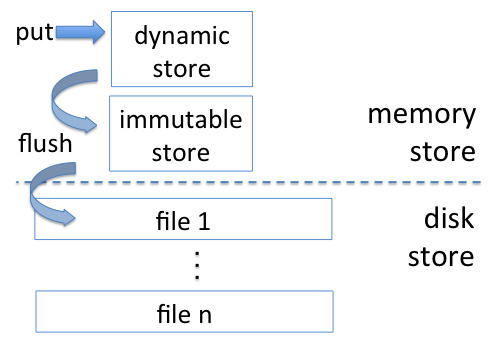
\includegraphics[width=0.85\columnwidth]{LSM} 
\caption{A typical LSM tree consists of a small memory store and a large disk store. 
Put operations update a dynamic data store. The memory store is double-buffered: 
a flush freezes the memory component, making it immutable, and creates a new dynamic store.
The immutable component is written to disk.}
\label{fig:LSM}
\end{figure}

\paragraph{LSM trees.}
% LSM trees - memory components
Many of the leading data stores today are organized as LSM trees, which collect writes in a memory store 
and periodically flush the memory into a disk store, as illustrated in Figure~\ref{fig:LSM}. 
The memory store is called \emph{MemStore} in HBase, and the disk store consists of multiple files
called \emph{HFiles} in HBase.
To allow puts to proceed in parallel with disk I/O, the memory store employs double buffering using two data structures: 
The first is a  \emph{dynamic store} absorbing puts, and the second is 
an \emph{immutable} previous version of the dynamic store, which is written to disk. 
Both data structures are sorted by key, as are the files in the disk store. 

% LSM puts and flushes
Put operations are directed to the MemStore.
When this store reaches a certain size limit, a flush occurs. 
Flush first freezes the current dynamic store, making it immutable, and creates a new empty dynamic one.
It then replaces the dynamic store with an empty one, and proceeds to write the immutable store as a new file to disk.
 To keep the number of files bounded, compactions merge multiple disk files into one, while eliminating redundancies 
 (deleted or overwritten items). 

% LSM gets
The get operation first checks the dynamic store, and if the key is not found there, proceeds to read the HFiles. 
Reads from different files are interleaved. 
To expedite reads, LSM trees use a large RAM cache. 

\paragraph{Memory organization.}
% Regions
Key-value stores achieve scalability by sharding data into units called \emph{regions}
(also referred to as \emph{tablets}~\cite{Chang2008, PNUTS2008} or \emph{partitions}).
HBase shards data by key-range.
Each HBase region and column family pair is managed as an independent LSM tree, with its own MemStore and HFiles.
%Partitioning provides {\em horizontal scalability} -- stretching the service across multiple servers.

% Memory store
The  memory store is traditionally implemented as a dynamic index over a collection of data items; 
for example,  HBase MemStore uses the standard Java concurrent skiplist\footnote{\small{\url{https://docs.oracle.com/javase/7/docs/api/java/util/concurrent/ConcurrentSkipListSet.html}}}).
Data is multi-versioned, i.e., every put creates a new immutable version of the data item it is applied to. 
%
This implementation suffers from two drawbacks. First, the use of a big dynamic data structure entails 
the abundance of auxiliary small objects and references, which inflate the in-memory index. 
%compared to its compact on-disk sibling, sorted array. 
The overhead is most significant when the managed objects
are small, i.e., the metadata-to-data ratio is big~\cite{Wu2015}. Second, the versioning mechanism makes 
no attempt to eliminate redundancies prior to flush, i.e., the store size  steadily grows, independently of the workload. 
This is especially wasteful for heavy-tailed distributions that are prevalent in production workloads~\cite{Devineni:2015}.

\paragraph{Distributed storage system and WAL.}
Distributed data stores like HBase consist of multiple \emph{storage nodes}, also called \emph{region servers}.
Production web-scale stores are comprised of thousands of such nodes, each managing
dozens of regions~\cite{hbase,Chang2008}. Each region server holds at least one \emph{write-ahead log (WAL)}. 
Puts are directed to the appropriate region server, which logs the update to WAL for persistence, and 
applies it to the appropriate region. 

HBase is layered on top of Hadoop File System (HDFS), which replicates all data for reliability and fault-tolerance,
making disk writes more expensive. Furthermore, HDFS uses large data blocks of 64MB, which lends itself to writing 
data in big chunks. HDFS supports heterogeneous storage devices, for example, it is possible to deploy the WAL over
HDD and the disk store files over SSD.








